% "acmsmall" is ACM's single-column journal format (TOMS, TOPLAS, JACM, ...). Use
% "acmlarge" for the larger page of some journals, "acmtog" for ACM Transactions on
% Graphics. Add "review,anonymous" for a double-blind submission; "nonacm" removes the
% ACM rights block for drafts or arXiv. ACM's journals take the final copy as a PDF
% from this same file, so keep the metadata commands below.
\documentclass[acmsmall]{acmart}
\usepackage{tikz}

% Journal and issue: the editorial office tells you the real values after acceptance.
\acmJournal{TOMS}
\acmVolume{1}
\acmNumber{1}
\acmArticle{1}
\acmMonth{1}
\acmYear{2026}
\acmDOI{10.1145/0000000.0000000}

% Rights and copyright: ACM e-mails the correct lines (licence or copyright) at acceptance.
\setcopyright{acmlicensed}

\begin{document}

\title{A Specific and Short Title for Your Journal Article}

\author{First Author}
\email{first.author@example.edu}
\orcid{0000-0000-0000-0000}
\affiliation{%
  \institution{Example University}
  \department{Department of Computer Science}
  \city{City}
  \country{Country}}

\author{Second Author}
\email{second.author@example.com}
\affiliation{%
  \institution{Example Lab}
  \city{City}
  \country{Country}}

% The running head of the published article; "et al." from three authors on.
\renewcommand{\shortauthors}{First Author and Second Author}

\begin{abstract}
Summarise the problem, the approach and the key result in about 150 to 200 words. An
abstract for an ACM journal stands alone: no citations and no references to sections.
\end{abstract}

% Generate these at https://dl.acm.org/ccs, choose the concepts that fit, and paste the result.
\begin{CCSXML}
<ccs2012>
 <concept>
  <concept_id>10002950.10003705.10003707</concept_id>
  <concept_desc>Mathematics of computing~Solvers</concept_desc>
  <concept_significance>500</concept_significance>
 </concept>
 <concept>
  <concept_id>10003752.10003809.10003716</concept_id>
  <concept_desc>Theory of computation~Design and analysis of algorithms</concept_desc>
  <concept_significance>300</concept_significance>
 </concept>
</ccs2012>
\end{CCSXML}
\ccsdesc[500]{Mathematics of computing~Solvers}
\ccsdesc[300]{Theory of computation~Design and analysis of algorithms}

\keywords{keyword one, keyword two, keyword three}

\maketitle

\section{Introduction}
State the problem, why it is hard and what you contribute. Cite with \verb|\cite|, for
example~\cite{knuth84}; the ACM reference format sets the style, so there is nothing
to configure. A journal article may be long, so give the reader a roadmap: Section~\ref{sec:method}
describes the method and Section~\ref{sec:eval} the evaluation.

\section{Method}\label{sec:method}
Describe the approach. Theorem-like environments are predefined by acmart.

\begin{theorem}\label{thm:bound}
  The algorithm terminates after at most $O(n \log n)$ steps.
\end{theorem}
\begin{proof}
  Give the proof here; the \texttt{proof} environment ends with the usual square.
\end{proof}

Equations are numbered automatically:
\begin{equation}
  T(n) = 2\,T(n/2) + n .
  \label{eq:recurrence}
\end{equation}

\subsection{Related algorithms}
Compare with earlier work such as Dijkstra's shortest path algorithm~\cite{dijkstra59}.

\section{Evaluation}\label{sec:eval}
Explain set-up, data and what Table~\ref{tab:results} and Figure~\ref{fig:scaling} show.
ACM places table captions above the table and figure captions below.

\begin{table}[ht]
  \caption{Example results (lower is better)}
  \label{tab:results}
  \begin{tabular}{lcc}
    \toprule
    Method & Time (ms) & Memory (MB) \\
    \midrule
    Baseline & 120 & 512 \\
    Ours & 85 & 430 \\
    \bottomrule
  \end{tabular}
\end{table}

\begin{figure}[ht]
  \centering
  % A small figure drawn in TikZ; replace with \includegraphics[width=0.6\linewidth]{fig.pdf}.
  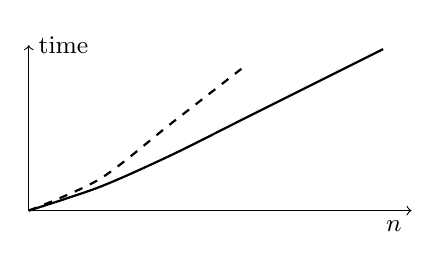
\begin{tikzpicture}[x=0.9cm,y=0.5cm]
    \draw[->] (0,0) -- (5.4,0) node[below left] {\small $n$};
    \draw[->] (0,0) -- (0,4.2) node[right] {\small time};
    \draw[thick] plot[smooth] coordinates {(0,0) (1,0.6) (2,1.4) (3,2.3) (4,3.2) (5,4.1)};
    \draw[thick,dashed] plot[smooth] coordinates {(0,0) (1,0.8) (2,2.2) (3,3.6)};
  \end{tikzpicture}
  \Description{Running time against input size n: the proposed method (solid) grows more slowly than the baseline (dashed).}
  \caption{Running time against input size (solid: ours, dashed: baseline).}
  \label{fig:scaling}
\end{figure}

\section{Conclusion}
One paragraph: what you showed and what comes next.

\begin{acks}
Funding bodies and people who helped, as one paragraph.
\end{acks}

\bibliographystyle{ACM-Reference-Format}
\bibliography{refs}

% After acceptance ACM also asks for \received{...}, \received[revised]{...} and
% \received[accepted]{...} here, with the dates of your submission history. They are left
% out because acmart warns about them (harmlessly) in a draft.

\end{document}
